\section{The Basilisk Platform}
\begin{frame}{The Basilisk Platform}
	\heading{Main Idea for the Platform}
	\begin{itemize}
		\item Continuously check for new triplestore releases or Pull Request
		\item Automatically perform a benchmark if a new release is found
		\item Store the benchmark results
	\end{itemize}
	
	%Idea, Overview, Services
	
	%Wie funktioniert?
	%Wie Komponenten?
\end{frame}

%\section{Architecture Overview}
\begin{frame}{Platform Architecture}
	\centering
	
	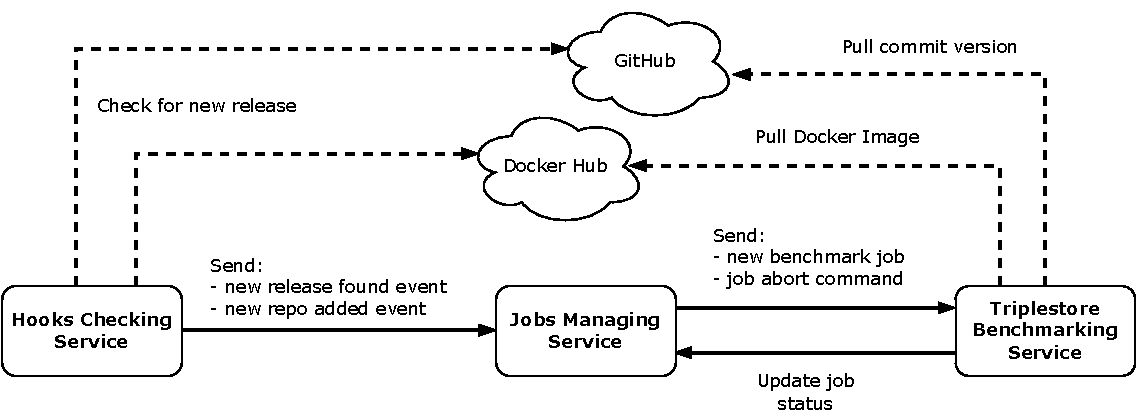
\includegraphics[width=1\textwidth]{images/basilisk/high-level-design-approach.pdf}
	
	\begin{itemize}
		\item User interaction via stateless REST endpoints
%		\begin{itemize}
%			\item All configurations are done on the REST endpoints at the JMS
%			\item HCS and TBS have one endpoint for starting or stopping
%		\end{itemize}
		\item Services communicate via a RabbitMQ message broker
	\end{itemize}
	
\end{frame}